\documentclass{article}
\usepackage{enumitem}
\usepackage{amsmath}
\usepackage[margin=1in]{geometry}
\usepackage{fancyhdr}
\usepackage{graphicx}

\pagestyle{fancy}
\fancyhf{}
\rhead{CS535, Fall 16}
\lhead{Lixuan Zhu (lz306)}
\rfoot{Page \thepage}
\begin{document}
\section{Problem 1}
\begin{enumerate}
\item
    In order to prove that $\Sigma$ is a valid covariance matrix, it is sufficient to show that $\Sigma$ is positive semi-definite. According to Sylvester's criterion, $\Sigma$ is positive definite if all of its leading principal minors must be positive, which is equivalent to all the diagonal elements obtained from Gaussian Elimination process must be positive. A proof of all the diagonal elements obtained by Gaussian Elimination process are positive is presented in Figure 1. Thus $\Sigma$ is a positive definite matrix and a valid covariance matrix.
    \begin{figure}[h]
        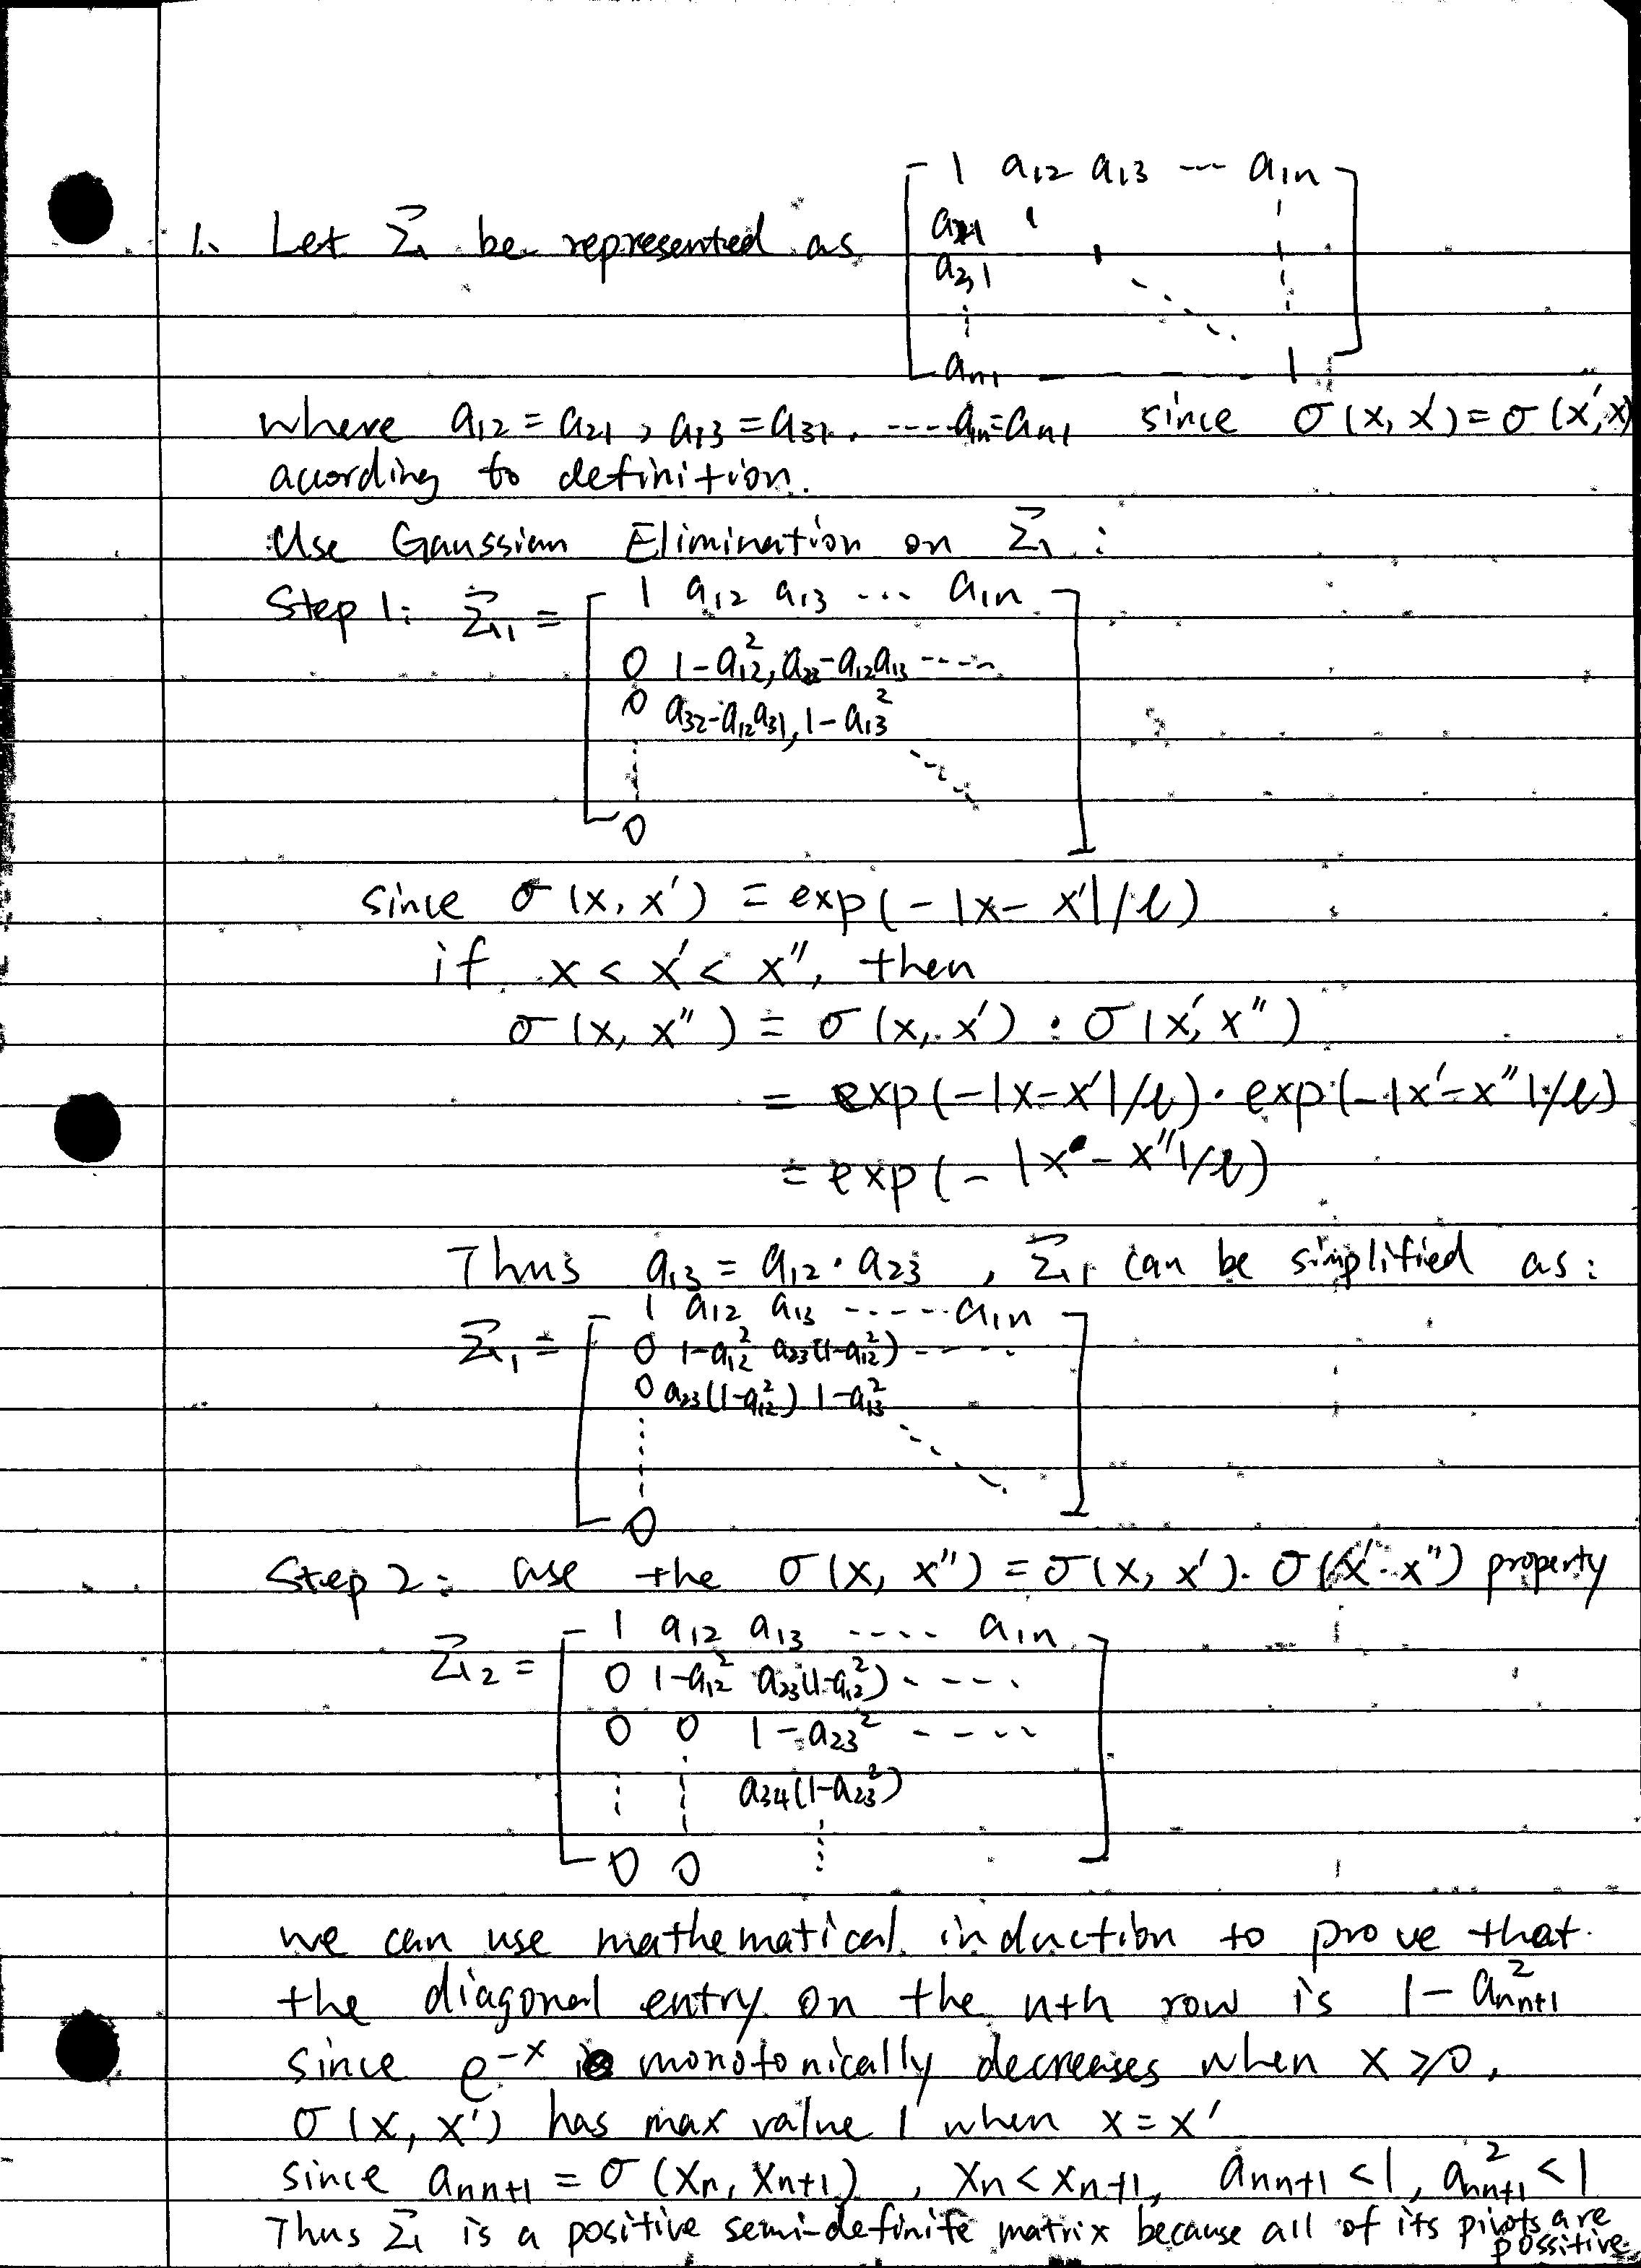
\includegraphics[width=1.0\linewidth]{fir.png}
        \caption{Problem 1.1}
    \end{figure}
\item
    Since all diagonal entries of the upper triangle matrix resulted from the Gaussian Elimination are positive, $det(\Sigma) > 0$ thus $\Sigma$ is invertible. Since $\Sigma$ is positive semi-definite as we proved previously, apply Cholesky decomposition we get $\Sigma = LL^T$, where $L$ is a lower triangular matrix with positive diagonal elements. In order to find $\Sigma^{-1}$, we first find $L^{-1}$ then $\Sigma^{-1} = L^{-T}L^{-1}$. The detailed process can be found in Figure 2 and 3.
    \begin{figure}[h]
        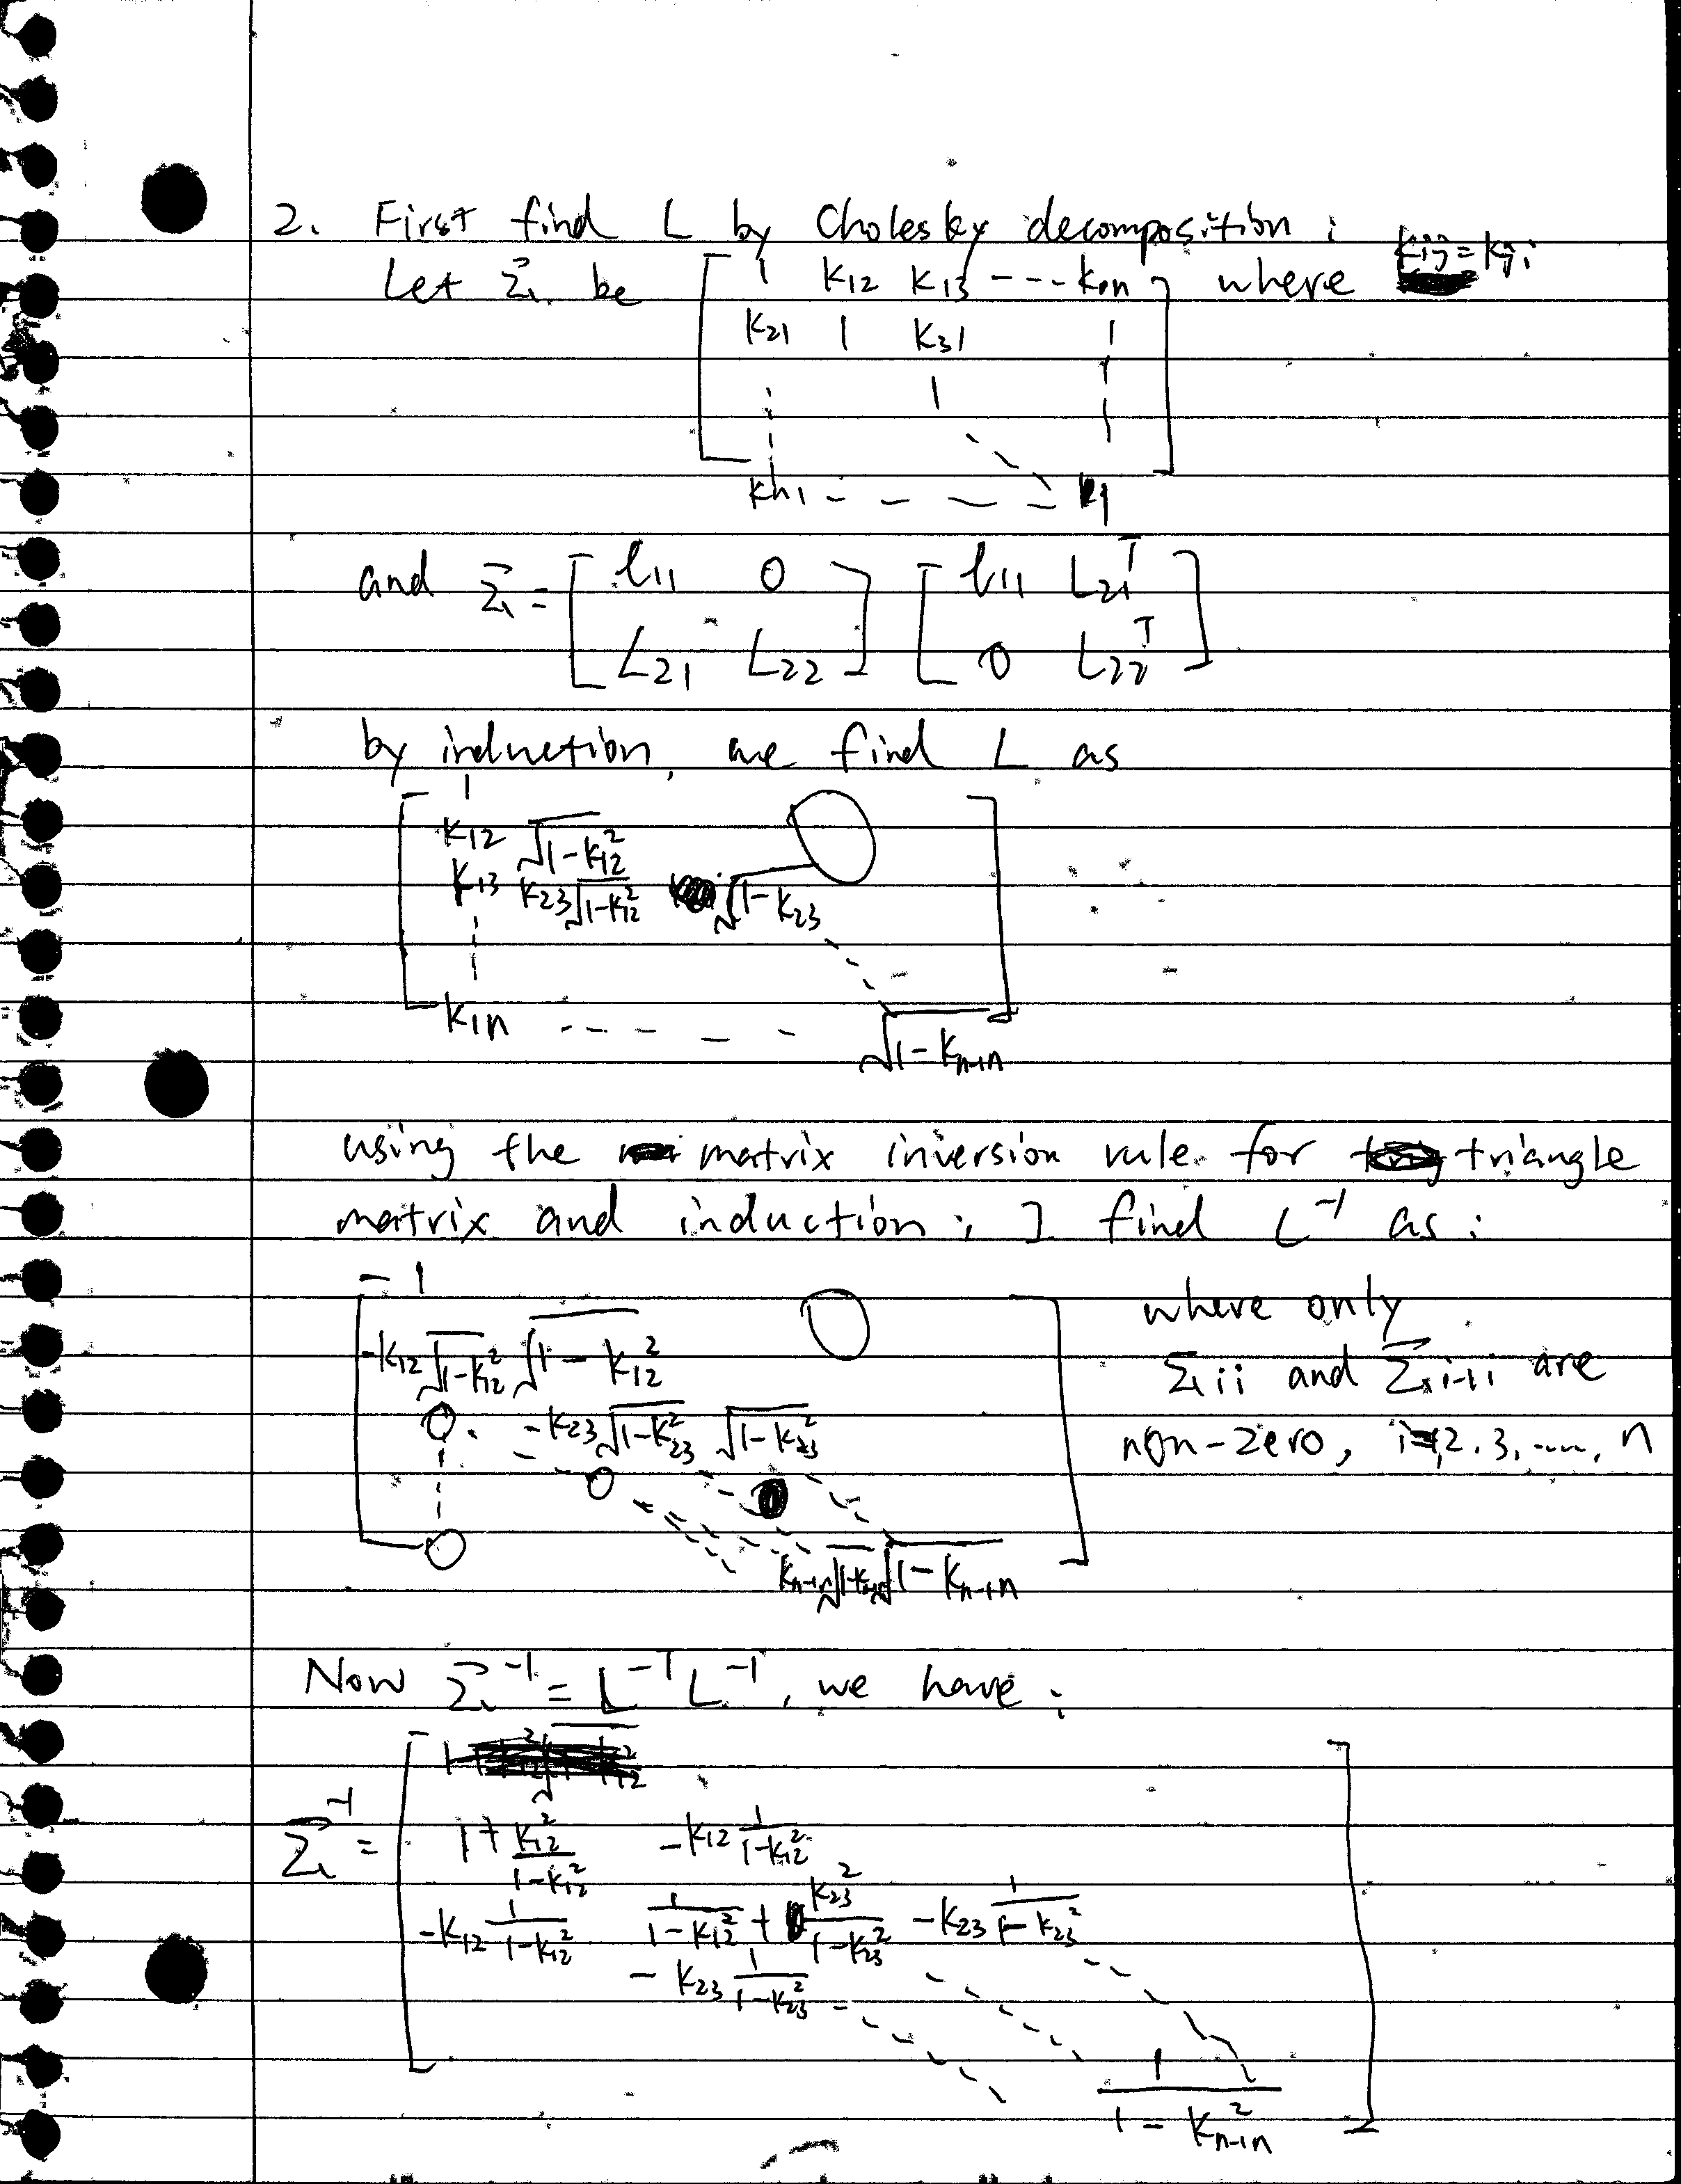
\includegraphics[width=1.0\linewidth]{sec.png}
        \caption{Problem 1.2}
    \end{figure}
    \begin{figure}[h]
        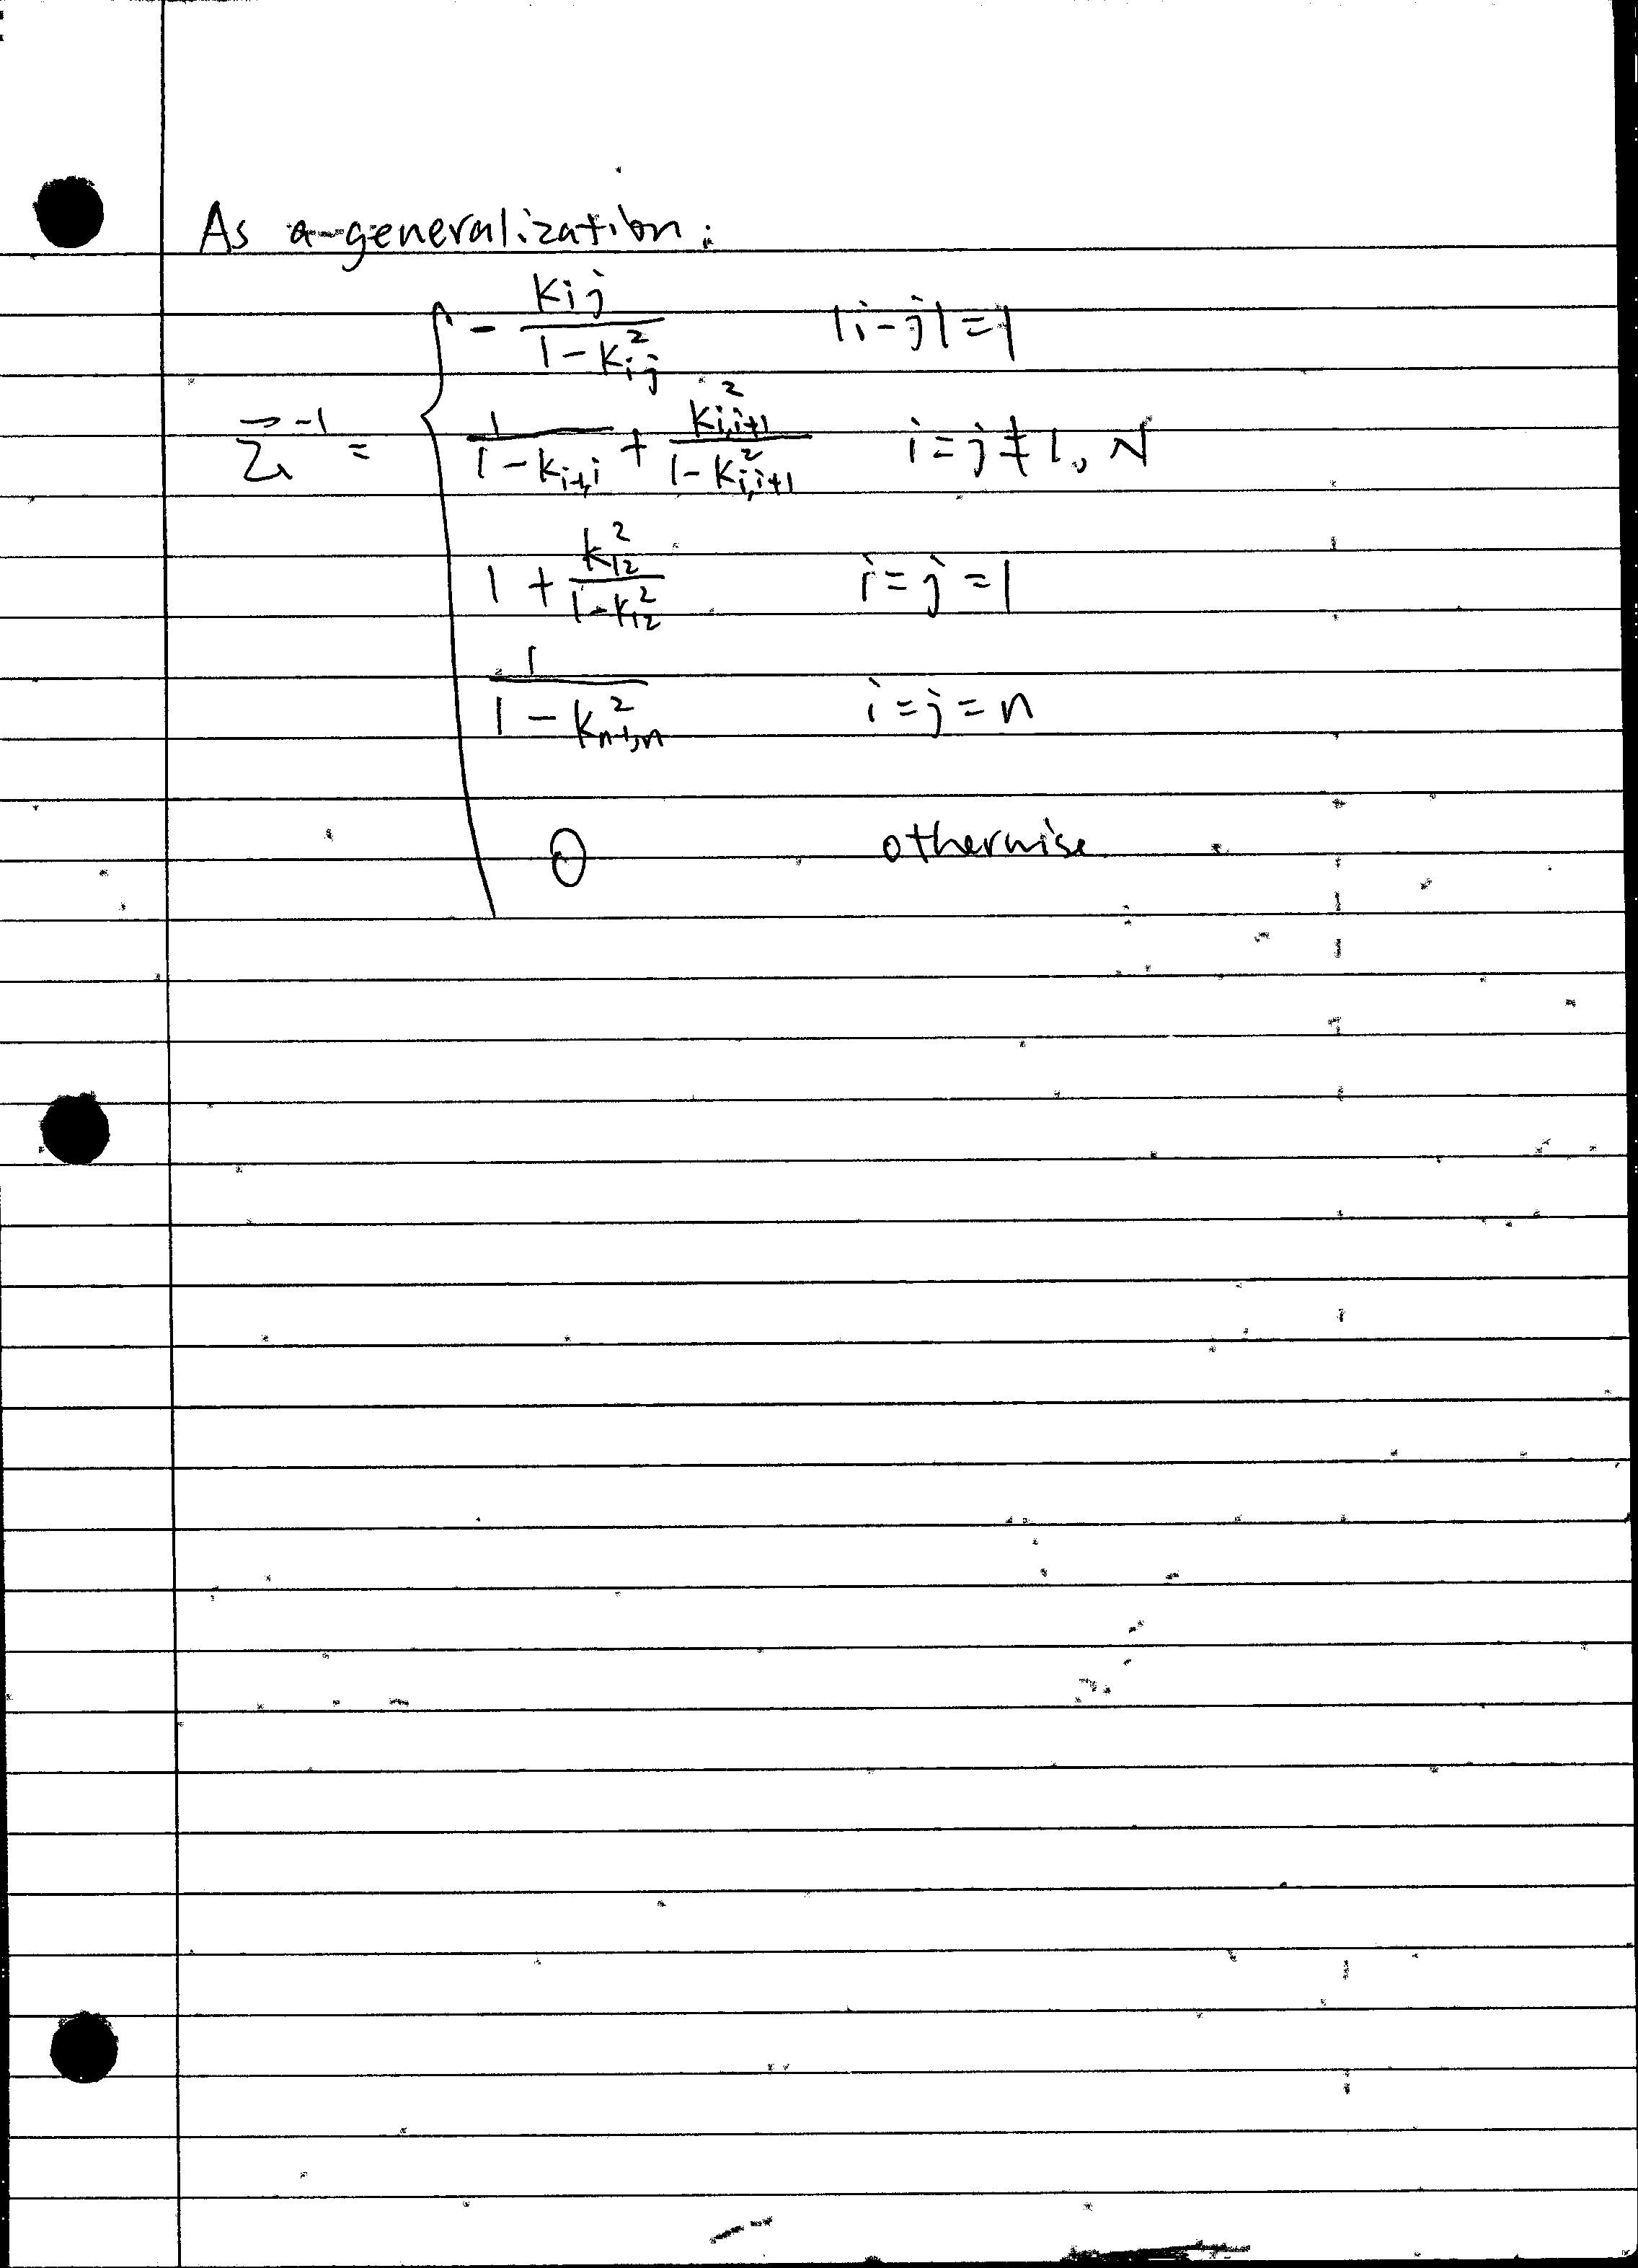
\includegraphics[width=1.0\linewidth]{gen.png}
        \caption{Problem 1.2}
    \end{figure}
\item
    According to the definition of statistical correlation:
    \begin{equation}
    \begin{split}
        \rho(y_i, y_j) &= \frac{\sigma(y_i, y_j)}{\sqrt{\Sigma^{y}_{ii}\Sigma^{y}_{jj}}}\\
                       &= \frac{exp(-|y_i - y_j|/l)}{\sqrt{\sigma(y_i, y_i)\sigma(y_j, y_j)}}\\
                       &= \frac{exp(-|y_i, y_j|/l)}{\sqrt{1*1}}\\
        &= exp(-|y_i, y_j|/l)
    \end{split}
    \end{equation}
\item
    Please refer to Figure 4.
    \begin{figure}[h]
        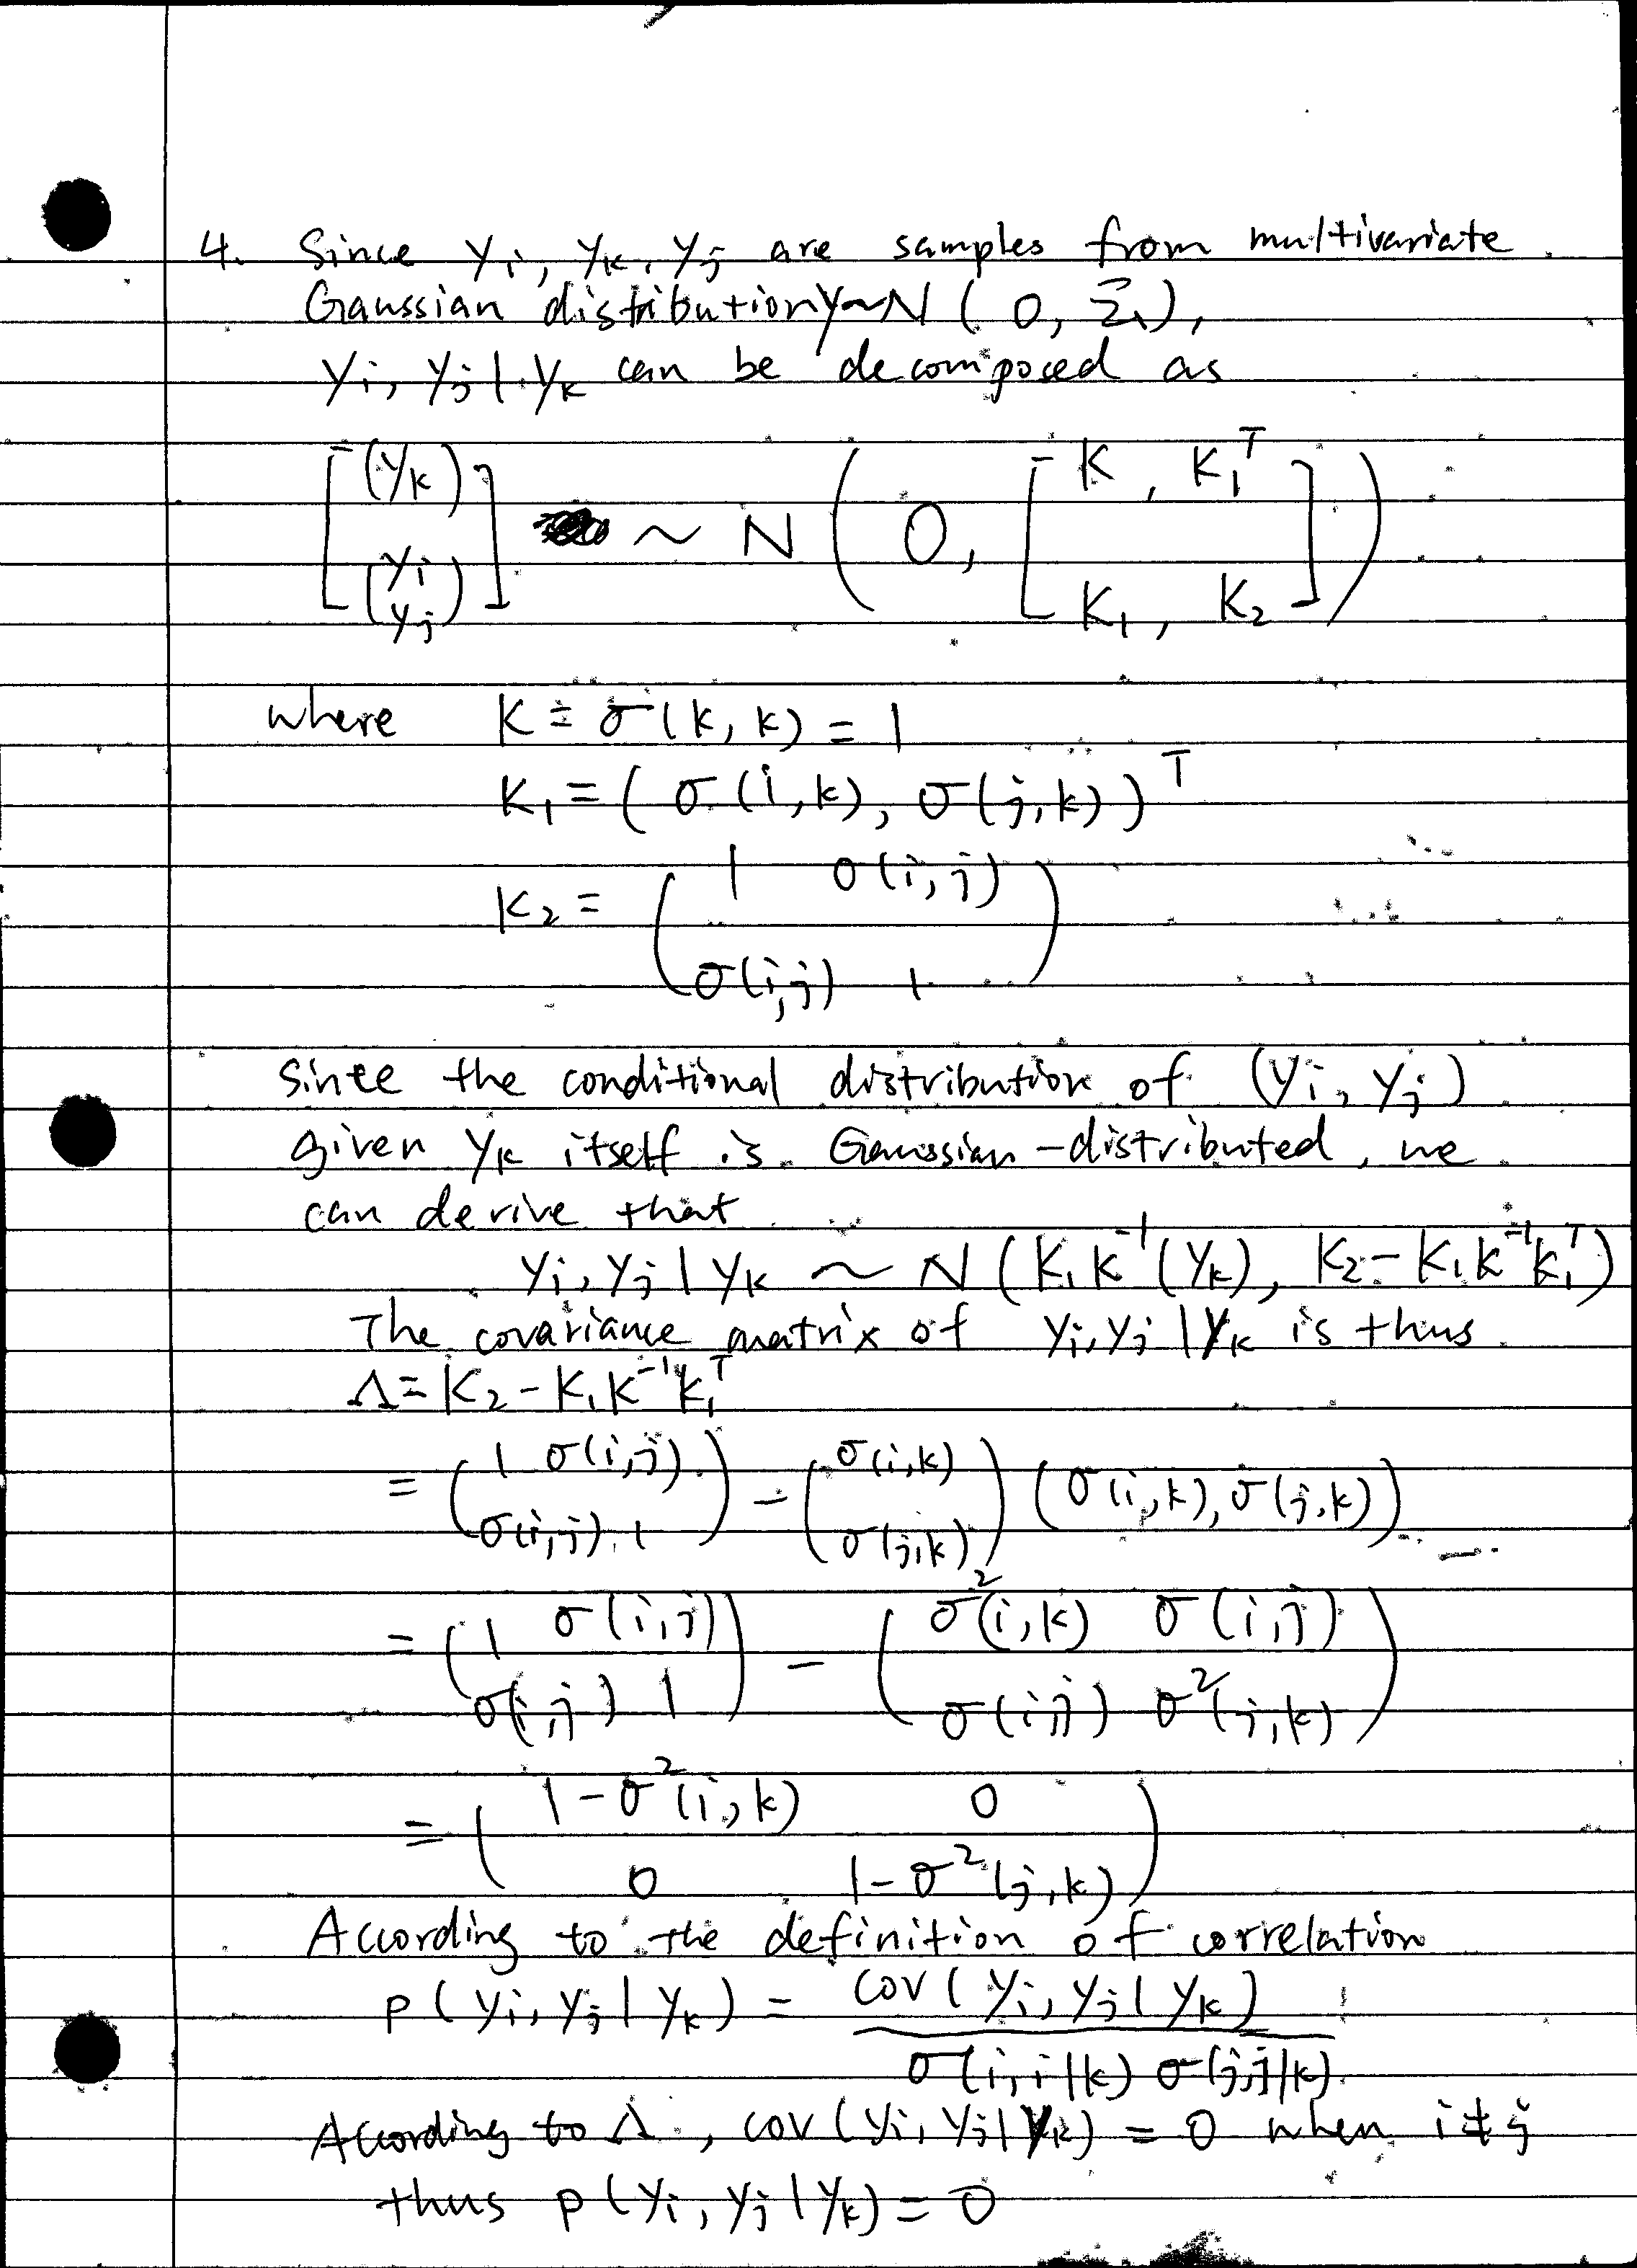
\includegraphics[width=1.0\linewidth]{four.png}
        \caption{Problem 1.4}
    \end{figure}
\item
    Please refer to Figure 5.
    \begin{figure}[h]
        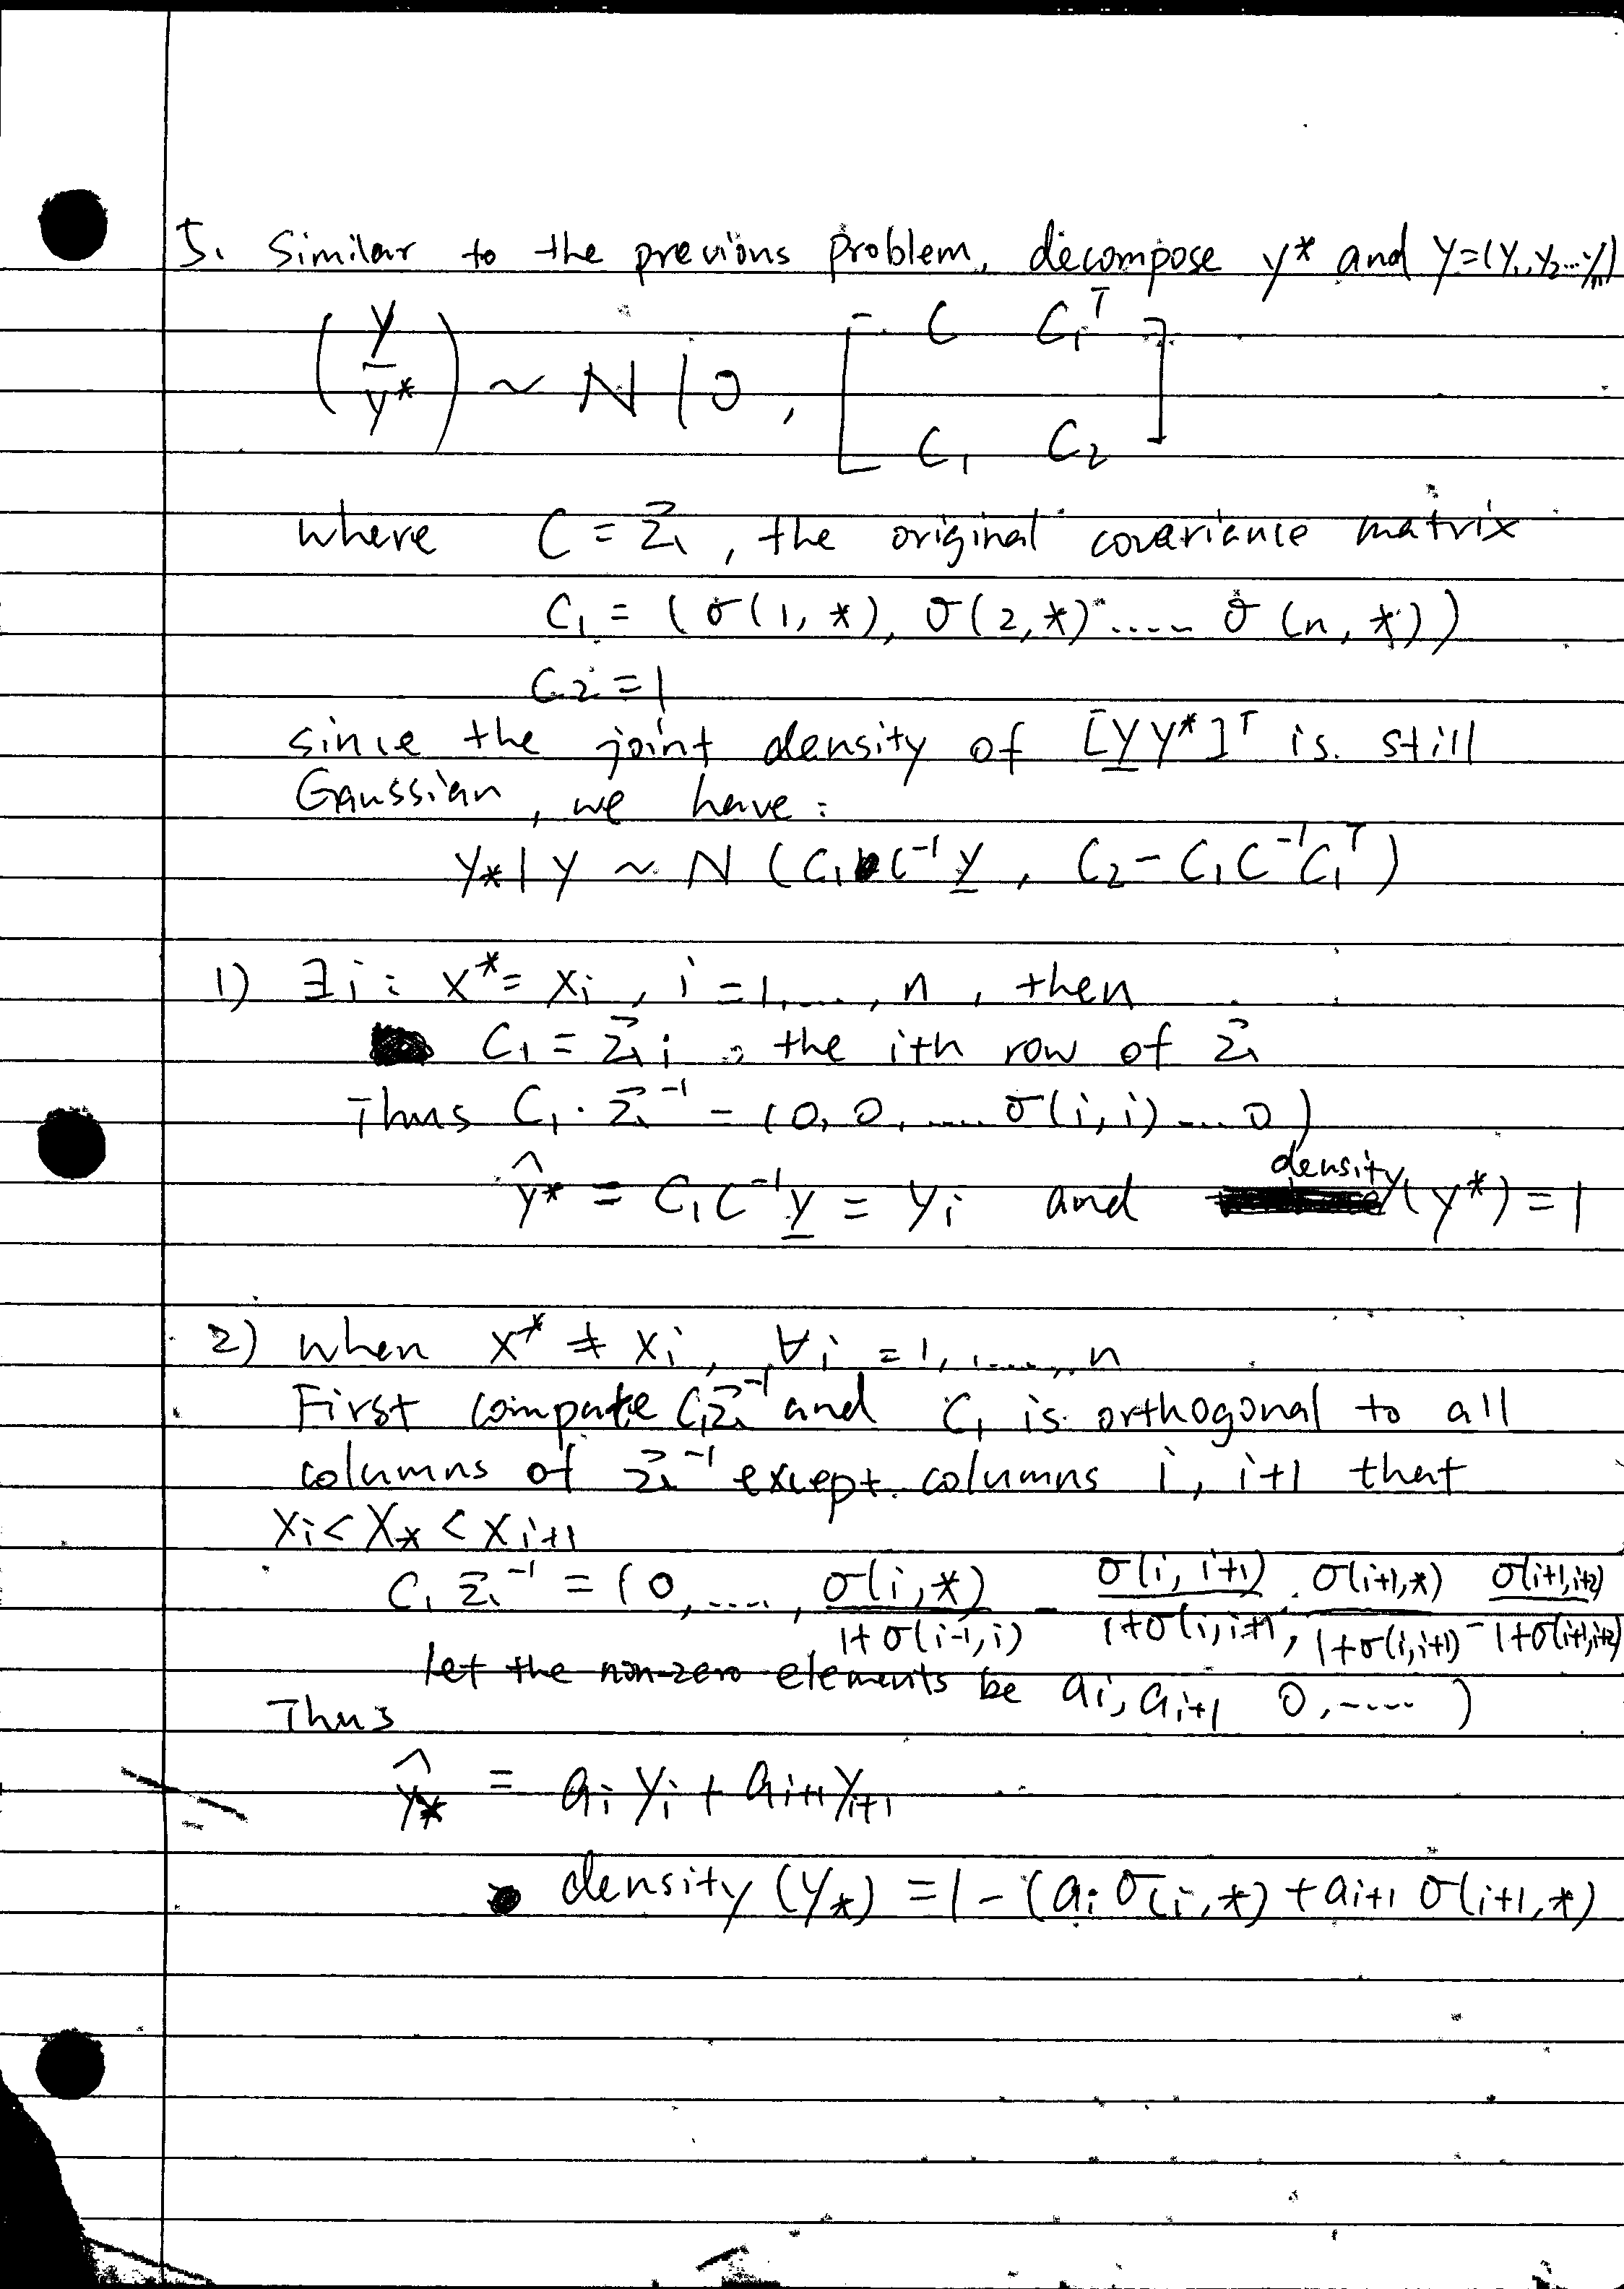
\includegraphics[width=1.0\linewidth]{five.png}
        \caption{Problem 1.5}
    \end{figure}
\item
    Assume the original $x_1 < ... < x_N$ is generated through uniform Gaussian distribution with zero-mean. First find the empirical covariance matrix $\Gamma$ from $y_1,.....,y_N$ which is an estimate of $\Sigma$. Then sample a set of $x_i$ from the multivariate Gaussian with zero-mean and covariance matrix $\Gamma$. This solution is not in closed form and not unique because the result of different sampling from the multivariate Gaussian is different.
\end{enumerate}
\section{Problem 2}
\begin{enumerate}
\item
    N/A
\item
    Maximize $log det\Theta - tr(S\Theta)$ subject to $||\Theta||_1 < t$, where $t > 0$ is a tuning factor. That is, maximize the Gaussian log-likelihood of the data subject to the constraint of $L_1$(lasso) penalty.
\item
    The optimization objective of PCA can be viewed from two different perscpectives. The first perspective is to find a low-dimensional subspace such that when the data is reconstructed from the subspace, the reconstruction error is minimized. The second perspective is to find linear projection such that the variance in the subspace is maximized. Compared to PCA, Graph Lasso method is not concerned with reconstructing the data but only concerned about preserving the maximum correlation information between data while keeping the inverse covariance matrix sparse in order to maintain computational convenience. The two methods are similar in that they both try to preserve as much information (variance and correlation respectively) from original data while keeping computation complexity managable. However, the two methods simplifies data in two different ways: reducing dimension and keeping inverse covariance matris sparse.
\item
    Let $f = logdet\Theta - tr(S\Theta) - tr(\Theta^2)$. Take the derivative of f:
    \begin{equation}
    \begin{split}
        \frac{d}{d\Theta}f = \frac{1}{det \Theta}\frac{d}{dX}det X - \frac{d}{dX} tr(\Theta(S-\Theta))
    \end{split}
    \end{equation}
\item
    The adjacency matrix $A$ and precision matrix $\Lambda$ are exactly the same except the diagonal of $A$ is consists of all $0$s while the diagonal of $\Lambda$ is consists of all $1$s. They are both sparse because $Pr(a_{ij} = 1)$ is relativly small thus most of the entries are $0$s. Thus the resulting adjacency graph is also sparse, in some cases some points are disconnected from all other points subject to initial samplingi, as can be observed from Figure 5. In contrast, the covariance matrix $\Sigma_0 = \Lambda_0^{-1}$ is relatively dense, as can be observed from the left most matrix in Figure 5.
    \begin{figure}[h]
        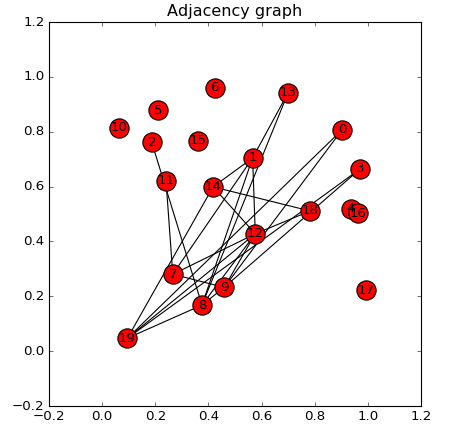
\includegraphics[width=.6\linewidth]{adj.png}
        \caption{Adjacency graph of matrix $A$.}
    \end{figure}
    \begin{figure}[h]
        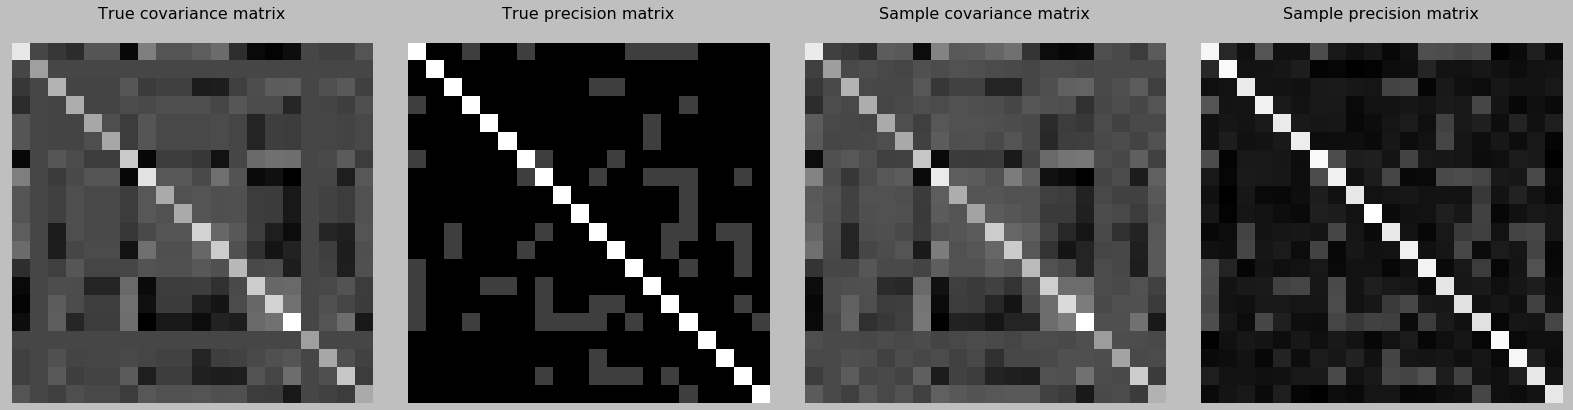
\includegraphics[width=1.15\linewidth]{true.png}
        \caption{"True" covariance/precision matrix and sample covariance/precision matrix.}
    \end{figure}
\item
    According to the sample covariance and precision in the right two matrices of Figure 6, the sample covariance is almost identical to "true" covariance matrix converted from true precision with slight differences since the sample covariance is estimated directly from the dataset. However, the sample precision matrix is much denser than "true" precision matrix because it is computed as the inverse of sample covariance. Slight difference between sample covariance and "true" covariance makes it impossible to reproduce the "true" precision matrix from sample covariance but it is easy to identify the 1 entries in "true" precision matrix from the sample precision matrix although the areas around those entries are blurry (with small non-zero entries).
\item
    \begin{figure}[h]
        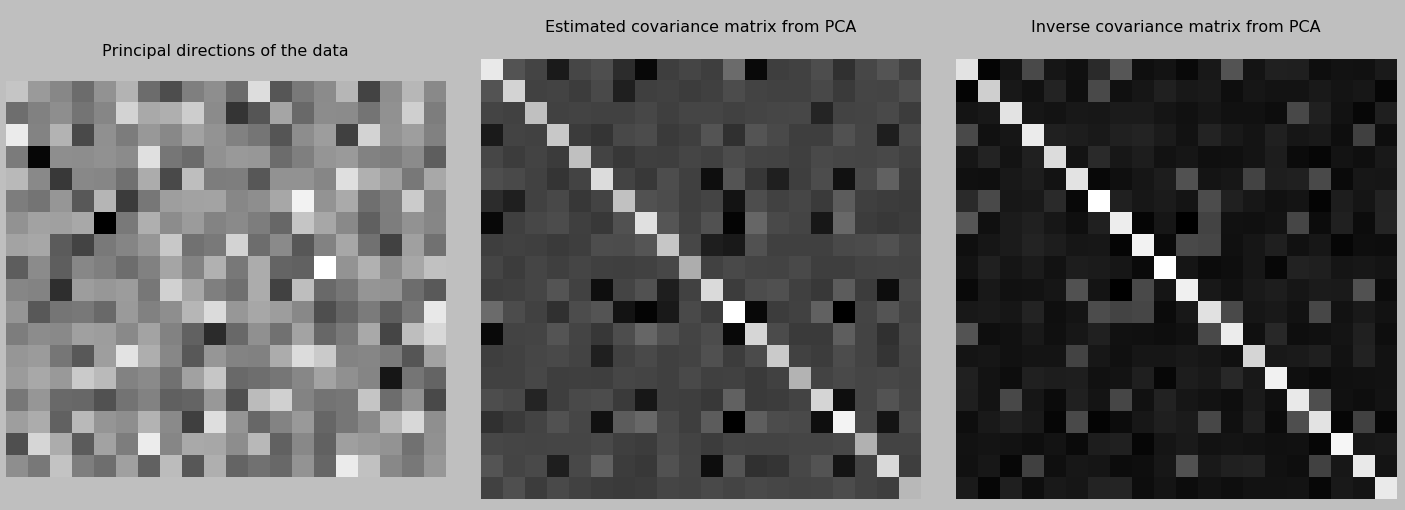
\includegraphics[width=1.1\linewidth]{prin.png}
        \caption{Principle directions and covariance/precision matrix of PCA.}
    \end{figure}
    \begin{figure}[h]
        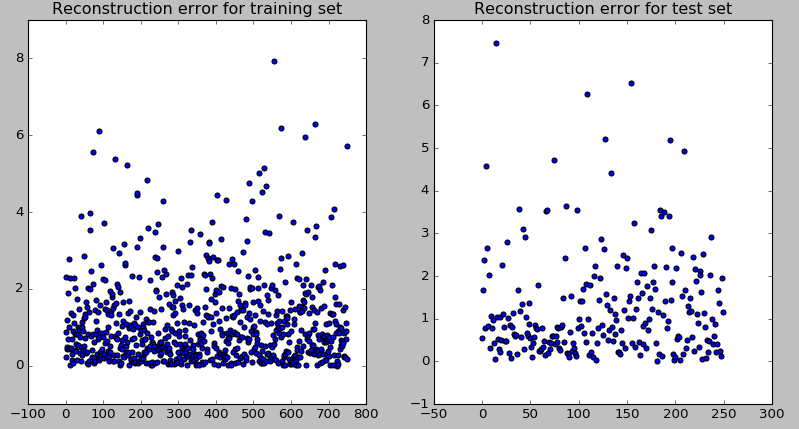
\includegraphics[width=.8\linewidth]{recon.png}
        \caption{Reconstruction errors of training/test sets.}
    \end{figure}
\item
\item
    The Graphical Lasso method estimates a sparse inverse covariance matrix by maximizing the Gaussian log-likelihood of the data. It controls the number of zeros (sparsity) in the inverse covariance matrix by imposing a $L_1$ (lasso) penalty. The algorithm finds the inverse covariance matrix by solving a lasso problem with coordinate descent procedure in each iteration until the resulting matrix converges. Graphical Lasso is much faster compared to other algorithms that solves the same problem.
    \par
    The reconstructed adjacency and covariance matrix are depicted in Figure 7.
    \begin{figure}[h]
        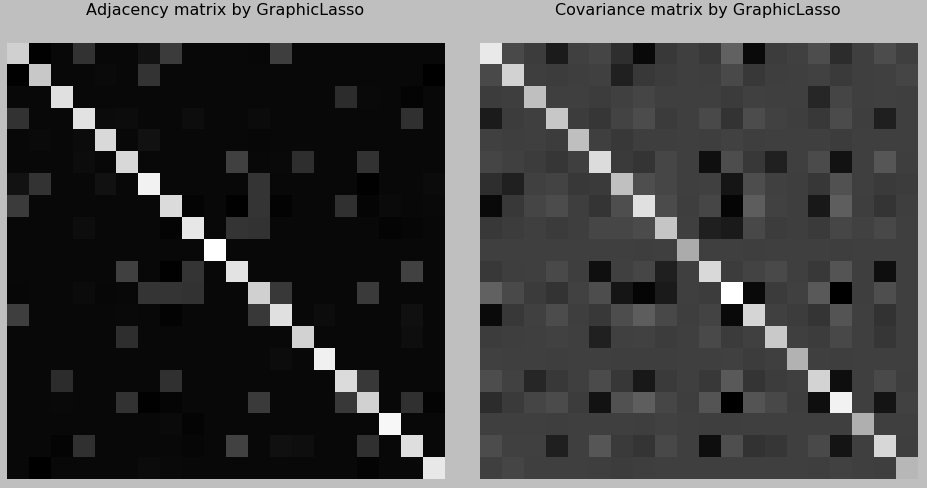
\includegraphics[width=1.0\linewidth]{lasso.png}
        \caption{Adjacency and covariance matrices estimated by Graphical Lasso.}
    \end{figure}
\item
    The first application is estimating the inverse covariance matrix of large-scale gene expression data from a multivariate Gaussian distribution. The second application is to learn the correlation of futures contract data with the estimated inverse covariance matrix and discover the graphical structure of how the price of commodities influence each other. The third application is to estimate the precision matrix of stocks in the US stock market in order to optimize portfolio management. PCA/PPCA cannot be used in these scenarios because true covariance matrix is hard to efficiently estimate in terms of large amount of data. The covariance matrix is large and dense because the data such as stocks and gene expression are closely related, thus the entries of covariance matrix cannot be forced to be sparse. Thus with Graphic Lasso it is much more efficient to estimate a sparse precision matrix and the performance is much faster than PCA/PPCA because of the usage of coordinate descent procedure. The primary usage of PCA/PPCA is to reduce the dimensionality of the data and preserve as much variance as possible, thus its not good for discovering correlation between data.
\end{enumerate}
\end{document}
